% arara: pdflatex: { shell: yes }



\PassOptionsToPackage{dvipsnames,cmyk}{xcolor}    % <Required for avoiding option clash for package xcolor
%-------------------------------------------------------------
% IMPORTANT (For mindmaps color transitions between nodes) If you load xcolor with option cmyk or rgb the colors match. 
% It seems that the default color model behaviour doesn't place nices with shadings.
% Explicitly using one of the two main ones apparently keeps xcolor more consistent.
% See:https://tex.stackexchange.com/questions/587568/mindmap-color-shading-between-root-node-and-children-not-using-correct-color  
%--------------------------------------------------------------                                             
% IMPORTANT: The dvipsnames colours are defined as CMYK colours, but by default, tikz produces shadings in RGB.
% This means the shading colours are silently converted from CMYK to RGB using a very simple formula from xcolor and so look completely different
% See: https://tex.stackexchange.com/questions/570799/tikz-shading-colors-does-not-match-with-others
%--------------------------------------------------------------
% IMPORTANT: The package tikz (by way of package pgfcore) loads the xcolor package.
% IMPORTANT: The standalone class with the option tikz also loads the tikz package (and configurates other settings so that it works as intended). 7
% The \usepackage{tikz} after \documentclass[tikz]{standalone} has no effect anymore.
% See: https://tex.stackexchange.com/questions/653681/how-to-use-xcolor-color-names-in-tikzpicture-style
%---------------------------------------------------------------
\documentclass[border=3.5pt]{standalone}  % see standalone package doc
\usepackage[utf8]{inputenc}
\usepackage{tikz}
\usetikzlibrary{mindmap,shadows}

% For avalilable dvipsnames see: https://www.overleaf.com/learn/latex/Using_colours_in_LaTeX



\definecolor{myGold}{cmyk}{0,0.18,0.99,0.01} 


\begin{document}
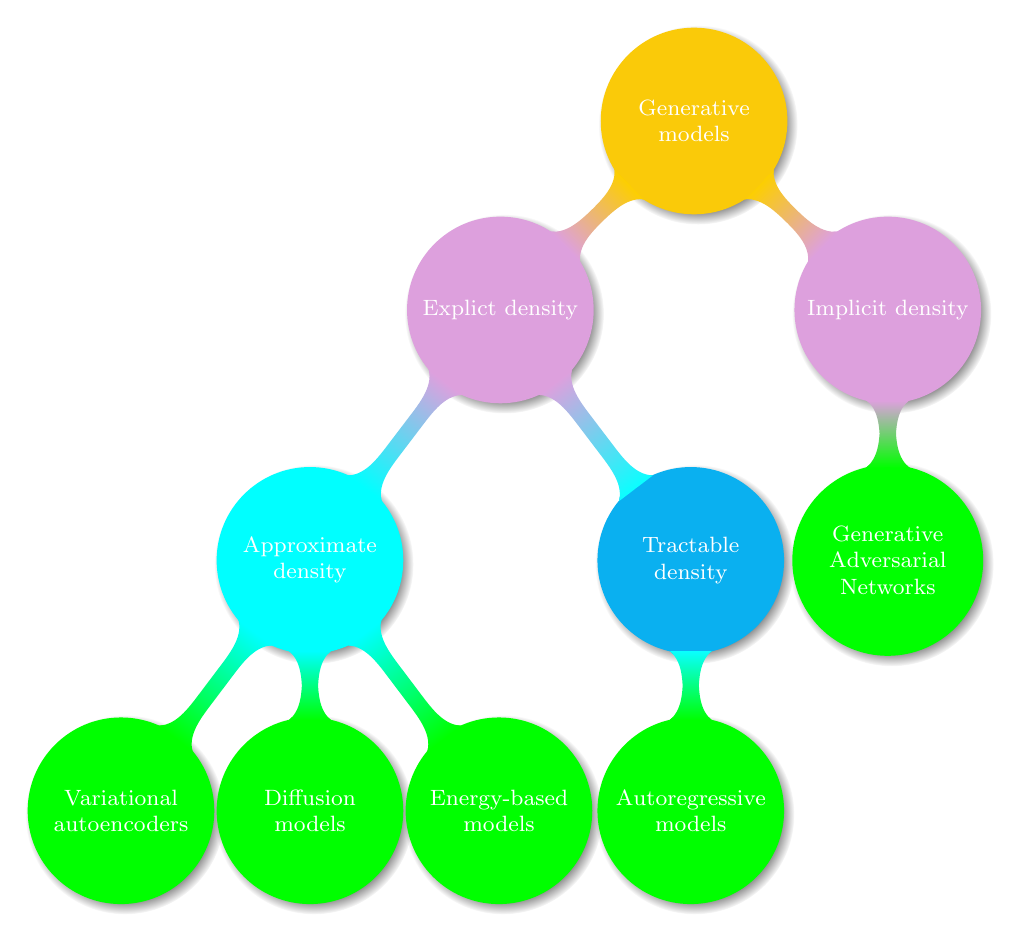
\begin{tikzpicture}[small mindmap,every node/.style={concept,circular drop shadow}, 
                    concept color=myGold,text=white,
                    level 1/.style={level distance=4cm, sibling distance=8.2cm},
                    level 2/.style={level distance=5.3cm, sibling distance=8.06cm},
                    level 3/.style={level distance=5.3cm, sibling distance=4cm}]                    
\node{Generative models}
    child [concept color=Plum, scale = 0.6]  { node {Explict density}
        child [concept color=Cyan] { node {Approximate density}
            child[concept color=green] { node {Variational autoencoders}}
            child[concept color=green] { node {Diffusion models}}
            child[concept color=green] { node {Energy-based models}}   
        }
        child [concept color=ProcessBlue] { node {Tractable density}
            child[concept color=green] { node {Autoregressive models}} 
        }
    }
    child [concept color=Plum,  scale = 0.6]{ node {Implicit density}
	    child [concept color=green] { node {Generative Adversarial Networks}}
    };
\end{tikzpicture}
\end{document}